
\chapter{APPENDIX} \label{ch:table appendix}

\vspace{-0.2in}

\section{Description of GOY Shell Model Runs and Table}

In most cases, we have forced the models in the first shell so that the inertial range forms on the ultraviolet side.  However, in run 2 from Table \ref{table: app GOY table}, we force in shell seven and observe an infra-red inertial range form.  Run 1 uses the parameters of \cite{Yamada} originally used.  This run is used as a control and to reproduce Pisarenko et. al. \cite{Pisarenko} work.  Run 2 is equivalent to Run 1 as far as the parameters are concerned.  However, in this run, we force in shell 6.  As a result, we see an infra-red inertial range.  We can apply the affine collapse to this data as well. This result is of interest in the light of Carl Gibson idea that the true cascade in turbulence is from small to large scales \cite{Gibson}. We start with small forcing in Run 3.  Here, the forcing is small enough that the solution is quasi-periodic and we have no inertial range.  We can observe this in the distribution of $u_n$.  In this particular case, the points were located in a ring that was centered at the origin (see Figure \ref{fig: circ symtrc}).   However, there is still circular symmetry about the origin in this case.

\begin{figure}[!htp]
    \begin{center}
        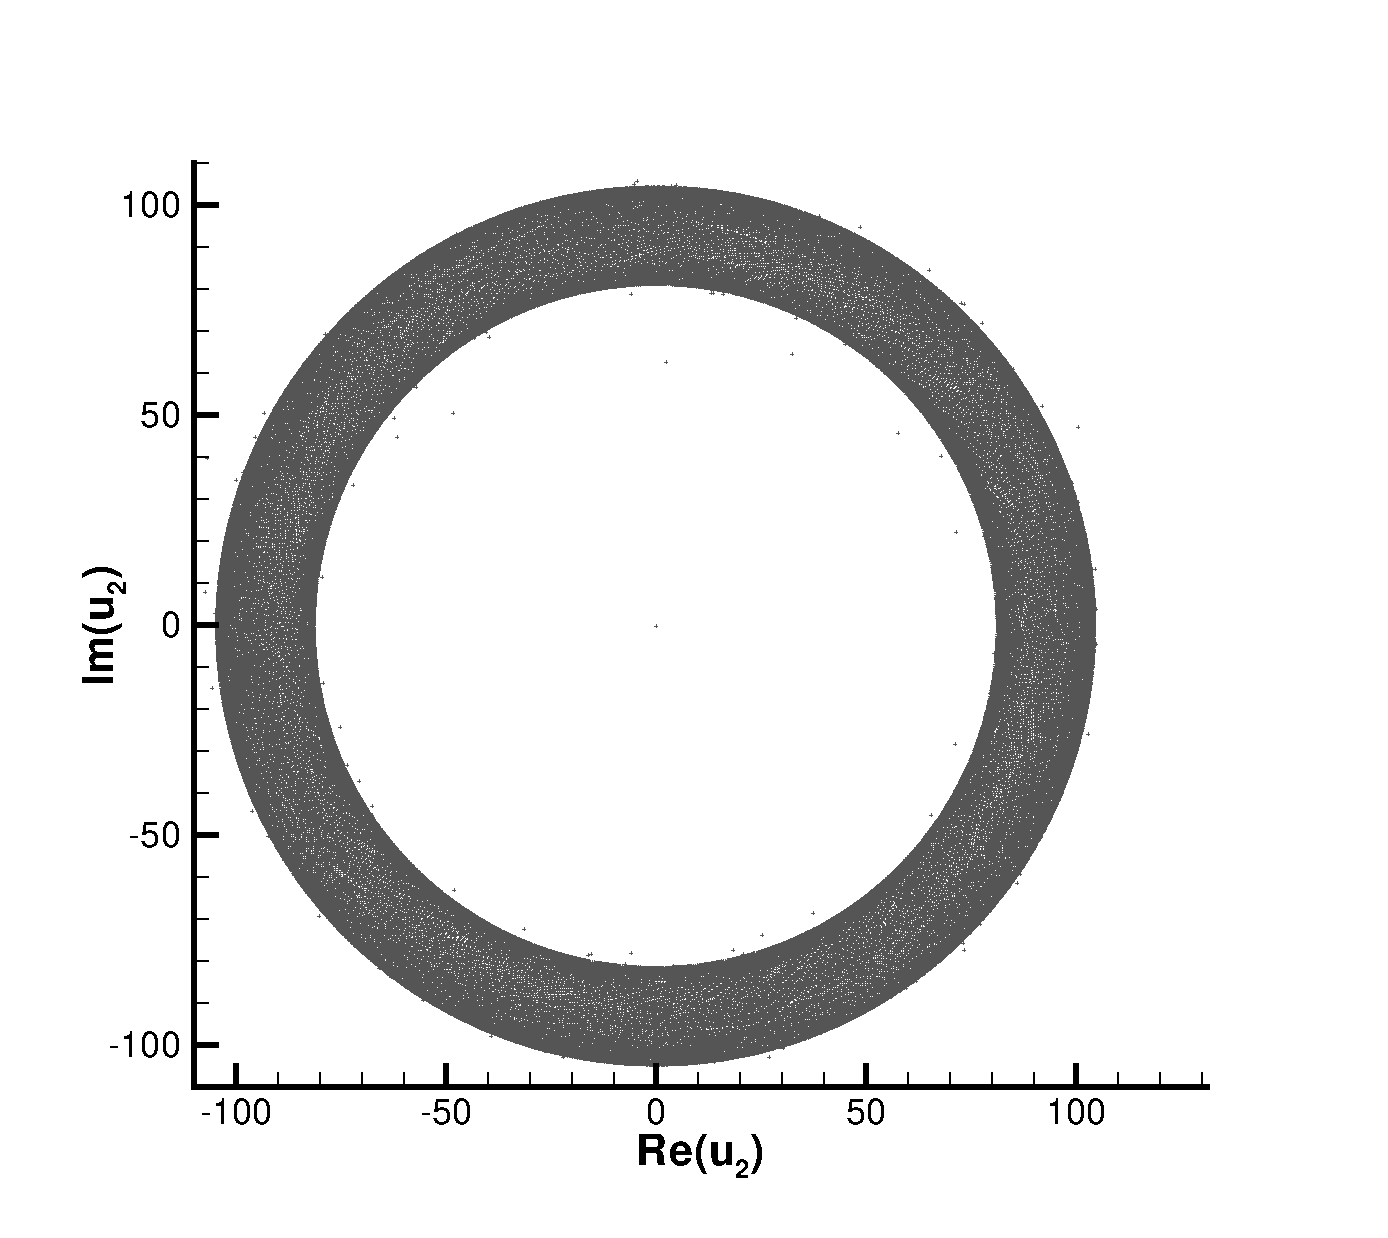
\includegraphics[width=4in]{ns_run10urui.eps}
    \end{center}
    \caption{Distribution of $u_i$. This plot displays the quasi-periodic nature of Run 3 for shell 10 (eps file).} \label{fig: circ symtrc}
\end{figure}

In order to obtain an inertial range which the new similarity theory requires, we increase the forcing for Run 4.  In Run 4, we still have virtually no inertial range.  We must increase the forcing further.  In Run 5, the model is chaotic and we have somewhat more of an inertial range.  Run 6 increases the forcing and the shell number, however we are not obtaining enough of an inertial range. In Run 7, we increase the forcing significantly.  The number of shells remains the same, but this time, we observe a distinct inertial range.  We want to observe how much forcing we can pump into the system before numerical problems arise.  Thus, we create Run 8 and Run 9.  Run 10 is at the limit of what is numerically possible with out model.  This run took four days to complete and is the longest run in the computation.  However, this run is not long enough to generate a statically significant ensemble for the smaller shell numbers.  Therefore, we have backed off in the forcing level and simulated a longer time series in Run 9.

%==========================================GOY Table runs=======================================
\begin{table}[!htp]
        \begin{center}
        \caption{Simulations with the GOY shell model with respective parameters. Run 1 uses the original GOY form found in (\ref{eq: classic goy}).  Runs 2-10 use the log polar form of GOY found in (\ref{eq:log polar goy}).}
        \begin{tabular}{||c|c|c|c|c|c|c||} \hline	
        \multicolumn{7}{|c|}{\emph{Types of Runs Considered for Collapse}} \\ \hline \hline
        Run $\#$    &$t_{end}$         &Forcing 			&$\nu$ 	   &$k_{0}$ &Forcing Shell &$\#$ Shells\\ \hline \hline
        1 & $2\times10^4$   &$(1+i)\times5\times10^{-3}$   &$10^{-7}$&$2^{-4}$ &$4$ &$22$\\
        2 &$1\times10^{-3}$ &$(1+i)\times2.048\times10^{16}$&$1$ 	   &$1$      &$7$ &$26$\\
        3 &$1\times10^{3}$ &$(1+i)\times10^{5}$		      &$1$	   &$1$	     &$1$ &$20$\\
        4 &$3\times10^{2}$ &$(1+i)\times10^{6}$	          &$1$	   &$1$	     &$1$ &$20$\\
        5 &$5\times10$ &$(1+i)\times10^{7}$		      &$1$	   &$1$	     &$1$ &$20$\\
        6 &$1\times10$ &$(1+i)\times10^{8}$  	      &$1$ 	   &$1$      &$1$ &$23$\\
        7 &$1\times10^{-3}$ &$(1+i)\times10^{12}$  	      &$1$ 	   &$1$      &$1$ &$23$\\
        8 &$1\times10^{-6}$ &$(1+i)\times10^{16}$  	      &$1$ 	   &$1$      &$1$ &$27$\\
        9 &$1\times10^{-8}$ &$(1+i)\times10^{20}$  	      &$1$     &$1$      &$1$ &$30$\\
        10&$1\times10^{-10}$ &$(1+i)\times10^{23}$	          &$1$	   &$1$      &$1$ &$36$\\
         \hline \hline
        \end{tabular}
        \end{center}
        \label{table: app GOY table}
\end{table}
%===============================================================================================


\section{Description of Sabra Shell Model Runs and Table}

Like the GOY shell model, the Sabra shell models are forced in the first shell so that the inertial range forms on the ultraviolet side.  However, in run 2 from Table \ref{table: app Sabra table}, forces in shell seven and we are able to observe an infra-red inertial range form. Run 1 uses the parameters of \cite{Yamada} originally used.  This run is used to illustrate the immediate differences between GOY and Sabra, i.e. oscillations in the inertial range.  Figure \ref{fig: ns_sfp} illustrates this.  Run 2 is equivalent to Run 1 in log polar form. The parameters are equivalent to \cite{Yamada} in the original evaluation.  However, in this run, we force in shell 7.  As a result, we see an infra-red inertial range. The affine collapse can be applied to this data as well.  The rest of the runs follow much the same as the GOY shell model.  We again focus on Run 9 for the same reasons as GOY.

%==========================================Sabra Table runs=======================================
\begin{table}[!htp]
        \begin{center}
        \caption{Simulations with the Sabra shell model with respective parameters. Run 1 uses the original Sabra form found in (\ref{eq:sabra}).  Runs 2-10 use the log polar form of Sabra found in (\ref{eq: log polar sabra}).}
        \begin{tabular}{||c|c|c|c|c|c|c||} \hline	
        \multicolumn{7}{|c|}{\emph{Types of Runs Considered for Collapse}} \\ \hline \hline
        Run $\#$    &$t_{end}$         &Forcing 			&$\nu$ 	   &$k_{0}$ &Forcing $n$ &$\#$ of $n$\\ \hline \hline
        1 &$2\times10^4$   &$(1+i)\times5\times10^{-3}$   &$10^{-7}$&$2^{-4}$ &$4$ &$22$\\
        2 &$1\times10^{-3}$ &$(1+i)\times2.048\times10^{16}$&$1$ 	   &$1$      &$7$ &$26$\\
        3 &$1\times10^{3}$ &$(1+i)\times10^{5}$		      &$1$	   &$1$	     &$1$ &$20$\\
        4 &$3\times10^{2}$ &$(1+i)\times10^{6}$	          &$1$	   &$1$	     &$1$ &$20$\\
        5 &$5\times10$ &$(1+i)\times10^{7}$		      &$1$	   &$1$	     &$1$ &$20$\\
        6 &$1\times10$ &$(1+i)\times10^{8}$  	      &$1$ 	   &$1$      &$1$ &$23$\\
        7 &$1\times10^{-3}$ &$(1+i)\times10^{12}$  	      &$1$ 	   &$1$      &$1$ &$23$\\
        8 &$1\times10^{-6}$ &$(1+i)\times10^{16}$  	      &$1$ 	   &$1$      &$1$ &$27$\\
        9 &$1\times10^{-8}$ &$(1+i)\times10^{20}$  	      &$1$     &$1$      &$1$ &$30$\\
        10&$1\times10^{-10}$ &$(1+i)\times10^{23}$	          &$1$	   &$1$      &$1$ &$36$\\
         \hline \hline
        \end{tabular}
        \end{center}
        \label{table: app Sabra table}
\end{table}
%=============================================================================================== 